\chapter{Resultados e Análise}

Os dados dos resultados foram exportados no formato csv, na pasta \texttt{``resultados\_caso\-\_regional''}, e para a exibição dos mesmos foi utilizada a ferramenta Power BI que é capaz de gerar diversos gráficos com certa praticidade e tendo arquivos .csv como entrada. Outros dados também foram impressos pelo terminal do python. 

Além disso, mapas geográficos interativos foram gerados utilizando a biblioteca \textit{Folium} do Python. Esses mapas foram dispostos em links online por meio do serviço de hospedagem da Netlify.

Foi gerado um arquivo do tipo csv com dados globais de cada modelo, o qual foi utilizado para a geração dos gráficos de comparação entre os modelos. Esse csv contém os seguintes dados dispostos nas seguintes colunas:

\begin{longtable}{|l|p{8.5cm}|}
\caption{Descrição das Colunas da Tabela de Comparação Entre Modelos} \label{tab:colunas_comparacao} \\
\hline
\textbf{Coluna} & \textbf{Descrição} \\ \hline
\endhead

\hline \endfoot

Modelo & Identificador do modelo matemático executado (1 ou 2). \\ \hline
Usa\_Penalidade & Indica se o cenário utilizou a penalidade na função objetivo. \\ \hline
Custo\_Medio\_Horas\_Por\_Dose & Métrica dada pela razão entre a soma dos custos ponderados de transporte (tempo multiplicado pelo volume de cada lote) e o total de doses movimentadas na rede. \\ \hline
Valor\_Funcao\_Objetivo & Valor numérico final obtido para a função objetivo correspondente após a otimização pelo \textit{solver} Gurobi. \\ \hline
Total\_Doses\_Movimentadas & Quantidade absoluta de doses de vacinas transportadas ao longo de todos os arcos ativos da rede de suprimentos. \\ \hline
Total\_Doses\_Faltantes & Somatório das variáveis de folga ($f_{pv}$), representando o déficit absoluto de indivíduos não atendidos em relação às metas dos postos. \\ \hline
Percentual\_Rodoviario & Percentual de uso do modal rodoviário. \\ \hline
Percentual\_Aereo & Percentual de uso do modal aéreo. \\ \hline
Tempo\_Maximo & O tempo logístico máximo registrado para que a última dose viável complete seu circuito físico, definindo o gargalo global ($L$). \\ \hline
Vacina\_Maior\_Tempo & O tipo de imunizante contra a Covid-19 que esteve associado ao maior tempo de trânsito ou restrição de expiração no gargalo global. \\ \hline
Rota\_Gargalo\_ij & Identificação do arco crítico direto (Origem $i \to$ Destino $j$) que registrou o maior tempo de trânsito no modal rodoviário. \\ \hline
Tempo\_Rota\_Gargalo\_ij & Custo (em horas) associado ao arco crítico rodoviário direto $i \to j$. \\ \hline
Doses\_Rota\_Gargalo\_ij & Volume de vacinas alocado e transportado através do arco crítico rodoviário direto $i \to j$. \\ \hline
Rota\_Gargalo\_ik & Identificação do arco crítico na primeira etapa do modelo integrado, ligando o município de origem $i$ ao centro estadual $k$ ($L_1$). \\ \hline
Tempo\_Rota\_Gargalo\_ik & Custo (em horas) associado ao arco crítico $i \to k$. \\ \hline
Doses\_Rota\_Gargalo\_ik & Volume de vacinas alocado e transportado através do arco crítico da etapa $i \to k$. \\ \hline
Rota\_Gargalo\_kj & Identificação do arco crítico na segunda etapa do modelo integrado, ligando o centro estadual $k$ ao município de destino $j$ ($L_2$). \\ \hline
Tempo\_Rota\_Gargalo\_kj & Custo (em horas) associado ao arco crítico $k \to j$. \\ \hline
Doses\_Rota\_Gargalo\_kj & Volume de vacinas alocado e transportado através do arco crítico da segunda etapa $k \to j$. \\ \hline
Rota\_Gargalo\_jp & Identificação do arco crítico na etapa intramunicipal final, ligando o município de destino $j$ ao posto de saúde $p$ ($L_3$). \\ \hline
Tempo\_Rota\_Gargalo\_jp & Custo (em horas) associado ao arco crítico final $j \to p$. \\ \hline
Doses\_Rota\_Gargalo\_jp & Volume de vacinas alocado e entregue ao posto de saúde crítico $p$ vindo do município $j$. \\ \hline
\end{longtable}

Também foram gerados outros arquivos csv's específicos para cada modelo, os quais foram utilizados para a geração dos gráficos de resultados individuais dos modelos.

Esse csv contém os seguintes dados dispostos nas seguintes colunas:

\begin{longtable}{|l|p{8.5cm}|}
\caption{Descrição das Colunas da Tabela de Detalhes da Execução de Um Modelo Específico} \label{tab:colunas_detalhes} \\
\hline
\textbf{Coluna} & \textbf{Descrição} \\ \hline
\endhead

\hline \endfoot

Modelo & Identificador do modelo matemático executado (1 ou 2). \\ \hline
Usa\_Penalidade & Indica se o cenário utilizou a penalidade na função objetivo. \\ \hline
ID\_Fluxo & Identificador único sequencial atribuído a cada fluxo de transporte ativo gerado pelo \textit{solver}. \\ \hline
Rota & Representação textual do arco de transporte no formato "Origem $\to$ Destino". \\ \hline
Tipo\_Rota & Classificação do arco logístico na estrutura da rede (ex: intermunicipal $i \to k$ ou $k \to j$, ou intramunicipal $j \to p$). \\ \hline
Origem & Nome da localidade de origem onde as doses foram despachadas. \\ \hline
Lat\_O & Coordenada geográfica de latitude do ponto de origem. \\ \hline
Lon\_O & Coordenada geográfica de longitude do ponto de origem. \\ \hline
Destino & Nome da localidade de destino final do arco de transporte. \\ \hline
Lat\_D & Coordenada geográfica de latitude do ponto de destino. \\ \hline
Lon\_D & Coordenada geográfica de longitude do ponto de destino. \\ \hline
Custo\_Horas & Custo (em horas) associado estritamente àquele arco de transporte. \\ \hline
Doses & Quantidade absoluta de doses de vacinas transportadas naquele fluxo específico. \\ \hline
Vacina & O tipo de imunizante contra a Covid-19 transportado na rota. \\ \hline
Modal & O modal de transporte utilizado para a movimentação da carga (Rodoviário ou Aéreo). \\ \hline
\end{longtable}


\section{Comparação entre Modelos}

\begin{figure}[H]
    \centering
    \caption{Tempo Máximo Por Modelo}
    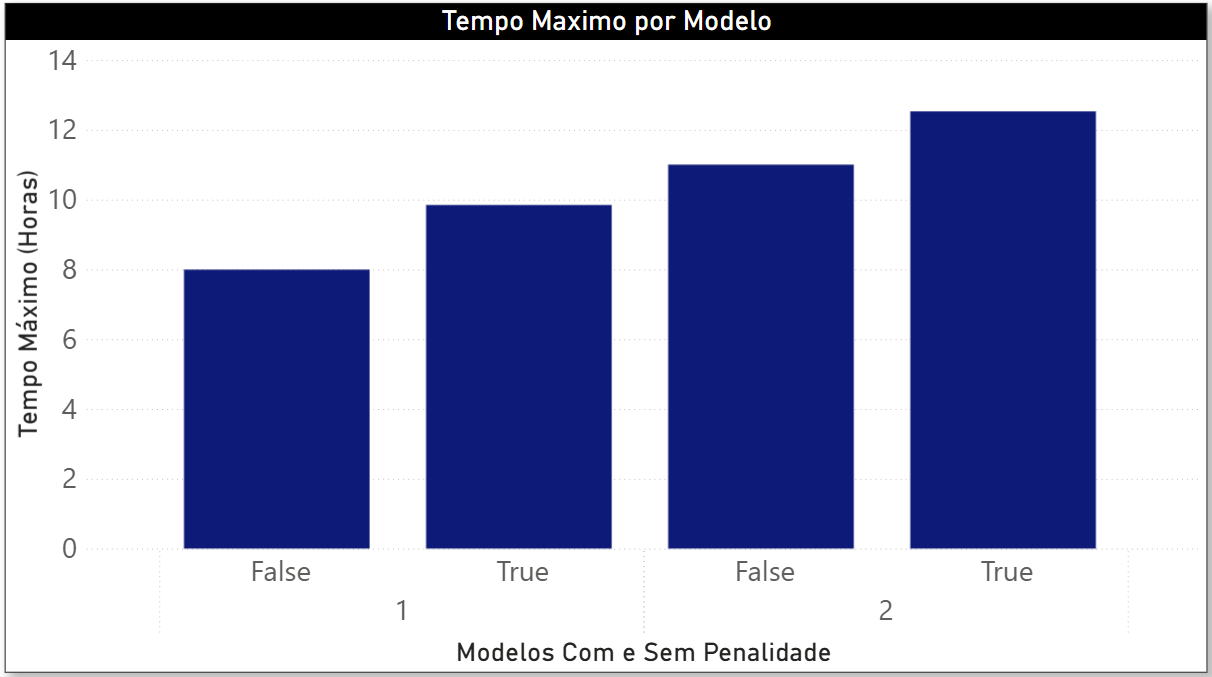
\includegraphics[width=16.0cm,height=9.0cm]{figuras/1-tempo_max_por_modelo.png} 
    \legend{Fonte: Elaborado pelo autor (2026)}
    \label{fig:grafico1_powerbi}
\end{figure}

Os tempos máximos são aproximados pelo valor do Limite Superior. 

Podemos verificar os modelos com penalidades possuem tempos maiores menores do que os modelos sem penalidades. Isso se deve ao fato de que a penalidade na função objetivo tem o efeito de priorizar o atendimento dos postos de saúde, mesmo que isso implique em rotas mais longas ou mais demoradas.

Observa-se também que as execuções do modelo 2 possuem um tempo maior do que as execuções do modelo 1, o que era esperado pelo modelo 2 incorporar mais etapas logísticas do que o modelo 1. Porém, agora conseguimos medir em quanto esse impacto é significativo.

Entre os modelos 1 e 2, ambos sem penalidade, a diferença entre os tempos é de aproximadamente 3 horas, isso significa que o modelo 2 tem um tempo $27\%$ maior.

Considerando os modelos ambos com penalidade, a diferença entre os tempos é de 2,7 horas. Isso significa que o modelo 2 tem um tempo $21\%$ maior.

\begin{figure}[H]
    \centering
    \caption{Valor da Função Objetivo Por Modelo}
    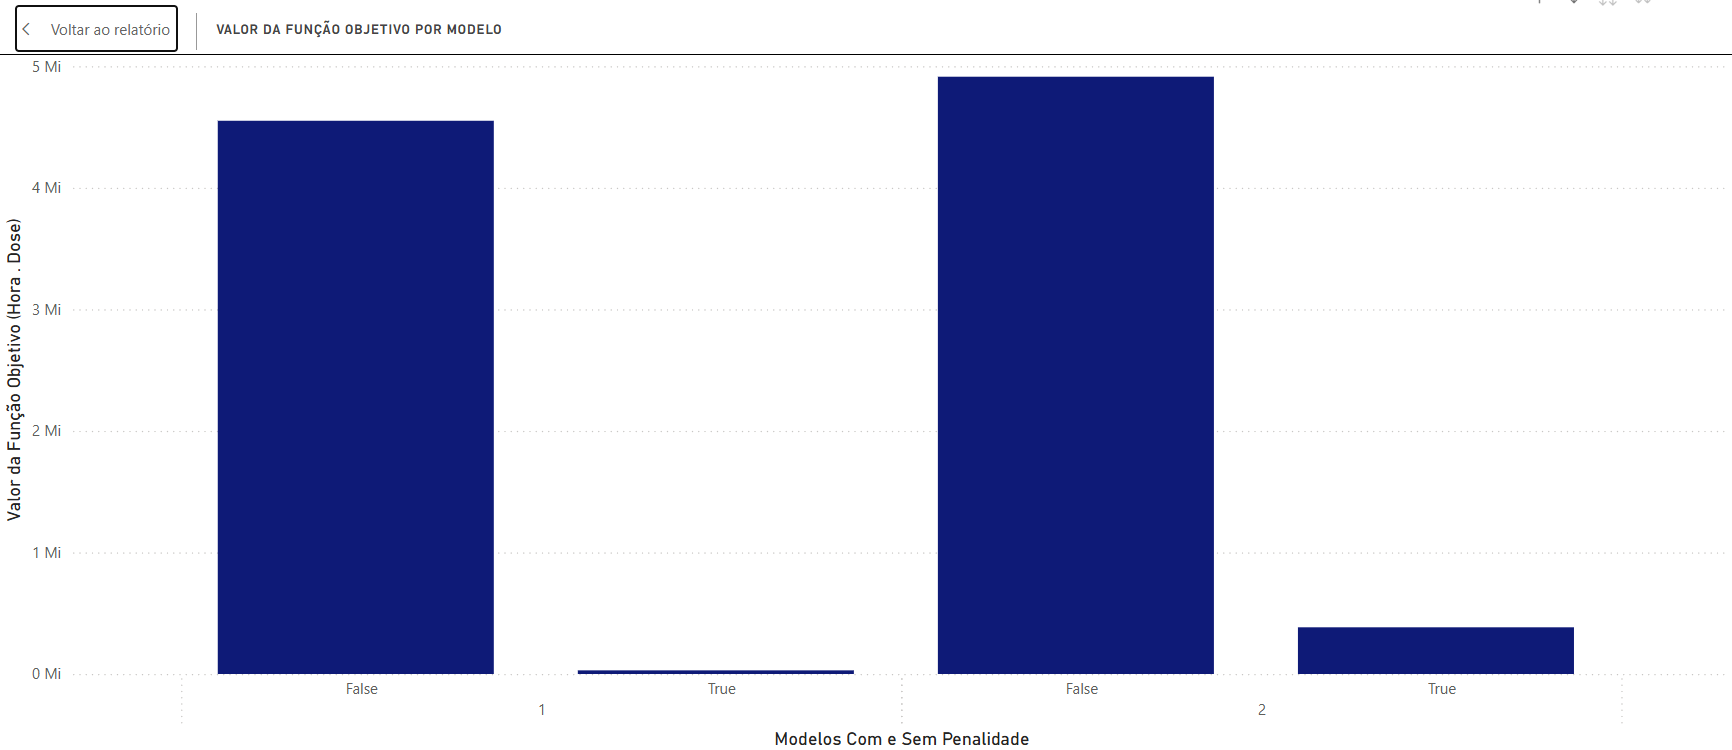
\includegraphics[width=16.0cm,height=9.0cm]{figuras/2-funcao_objetivo_por_modelo.png} 
    \legend{Fonte: Elaborado pelo autor (2026)}
    \label{fig:grafico2_powerbi}
\end{figure}

Este gráfico denota uma grande diferença no valor da função objetivo entre um modelo sem penalidade e sua versão com penalidade, pois o modelo com penalidade é severamente punido, por diversas vezes, a cada hora que uma vacina com validade curta passa em trânsito.

\begin{figure}[H]
    \centering
    \caption{Custo Médio (Em Horas) por Dose Por Modelo}
    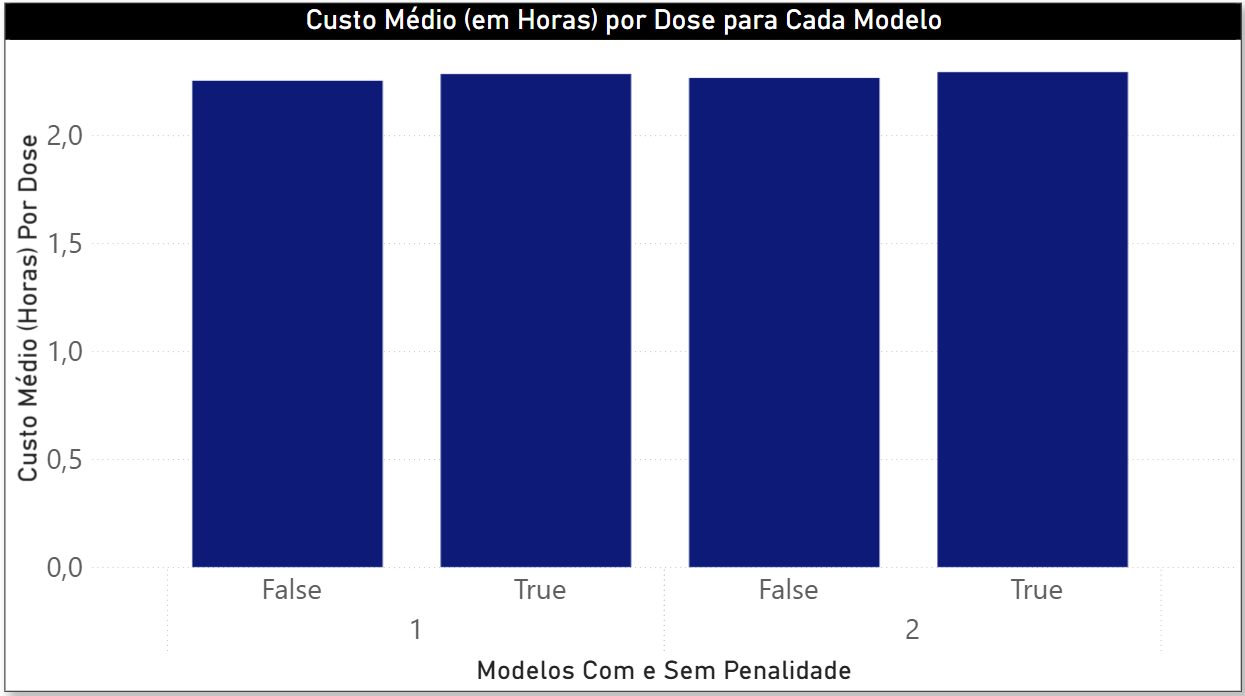
\includegraphics[width=16.0cm,height=9.0cm]{figuras/3-custo_medio_por_dose_por_modelo.png} 
    \legend{Fonte: Elaborado pelo autor (2026)}
    \label{fig:grafico3_powerbi}
\end{figure}

Para a obtenção deste gráfico, gerou-se uma média ponderada do custo em horas utilizando a quantidade de doses como peso multiplicador. Embora a penalidade ative rotas intermunicipais muito mais longas (de até 8 horas) para escoar lotes críticos, a média global permanece estável. Essa estabilidade matemática ocorre porque a etapa intramunicipal ($j \to p$) concentra a grande maioria das entregas (cerca de 70\% a 75\% da matriz) com grandes quantidades de doses por entrega. Assim, o volume massivo de vacinas transportadas localmente em tempos curtos dilui o peso das viagens extremas de longa distância, ancorando o custo médio final.

\begin{figure}[H]
    \centering
    \caption{Total de Doses Movimentadas Por Modelo}
    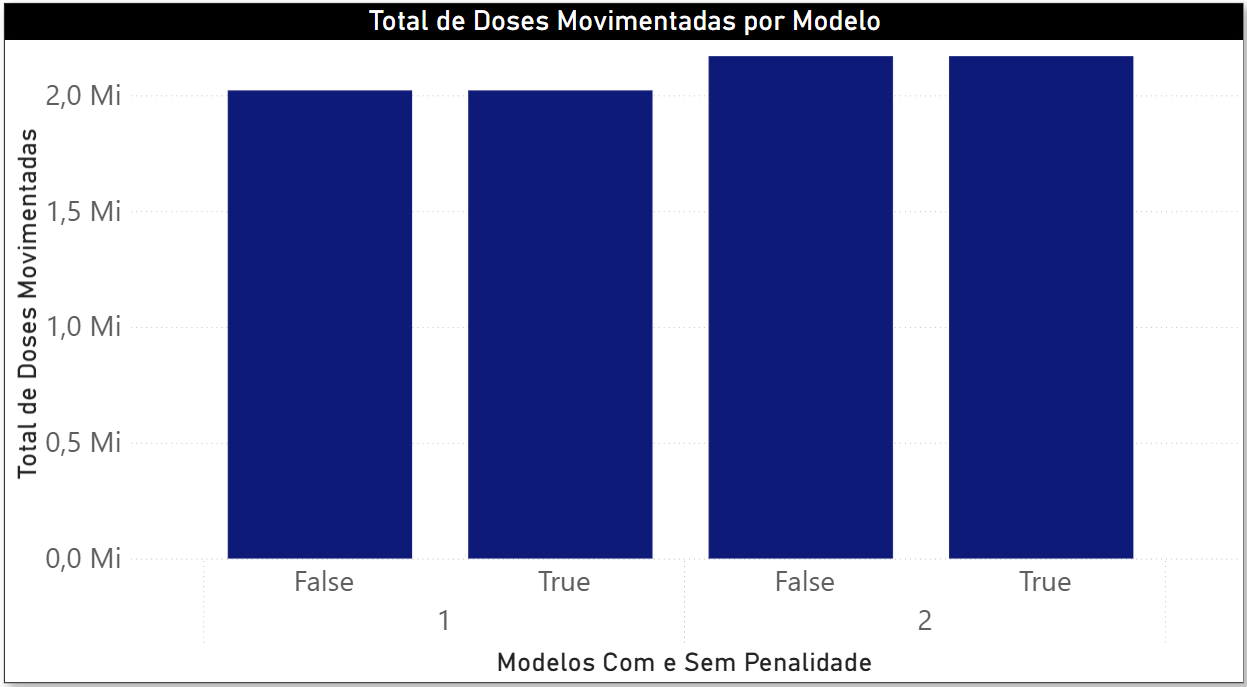
\includegraphics[width=16.0cm,height=9.0cm]{figuras/4-doses_movimentadas_por_modelo.png} 
    \legend{Fonte: Elaborado pelo autor (2026)}
    \label{fig:grafico4_powerbi}
\end{figure}

O total de doses movimentadas foi aumentado conforme mais etapas logísticas tinha o modelo. O modelo 2 apresentou o maior valor de doses movimentadas.

\begin{figure}[H]
    \centering
    \caption{Percentual de Uso dos Modais}
    
\includegraphics[width=16.0cm,height=9.0cm]{figuras/6-percentual_modais.png} 
    \legend{Fonte: Elaborado pelo autor (2026)}
    \label{fig:grafico5_powerbi}
\end{figure}

Nos modelos, há predominância do modal rodoviário.

Quase não há diferença nas porcentagens quando comparamos um modelo sem penalidade e sua versão com penalidade.

\section{Resultados Individuais dos Modelos}

Além da comparação entre os modelos, também é possível analisar o que acontece dentro de cada modelo de forma independente dos demais.

\subsection{Resultados do Modelo 1}

\begin{figure}[H]
    \centering
    \caption{Os 10 Maiores Tempos Por Rota - Modelo 1}
    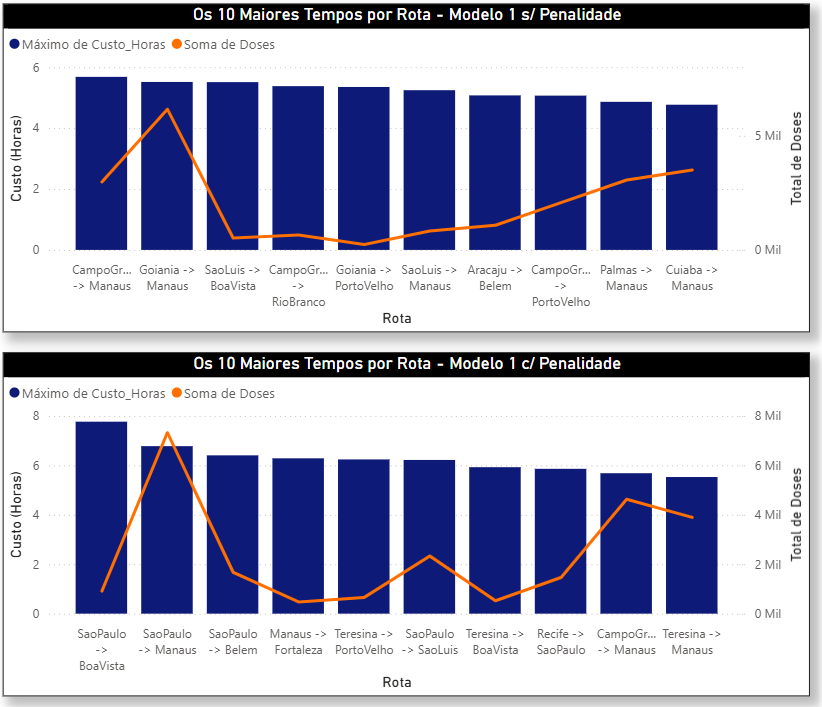
\includegraphics[width=16.0cm,height=12.5cm]{figuras/9-maiores_tempos_mod1.png} 
    \legend{Fonte: Elaborado pelo autor (2026)}
    \label{fig:grafico10_powerbi}
\end{figure}

No cenário sem penalidade, os maiores tempos de rota concentram-se em eixos que interligam capitais do Centro-Oeste e Nordeste em direção a Manaus (ex: Campo Grande $\to$ Manaus, Goiânia $\to$ Manaus, São Luís $\to$ Manaus), com tempos estabilizados na faixa de 5 a 6 horas.

No cenário com penalidade, o Gurobi altera completamente o conjunto. Surgem eixos de longuíssima distância partindo do Sudeste, como por exemplo São Paulo $\to$ Boa Vista, São Paulo $\to$ Manaus e São Paulo $\to$ Belém. Na presença da penalidade, o teto do eixo vertical de custos em horas sobe de 6 horas para 8 horas.

O trajeto irregular da linha laranja (Soma de Doses) em ambos os cenários confirma que não há proporcionalidade direta entre o tempo de voo e a quantidade de vacinas transportada.

\begin{figure}[H]
    \centering
    \caption{Os 10 Menores Tempos Por Rota - Modelo 1}
    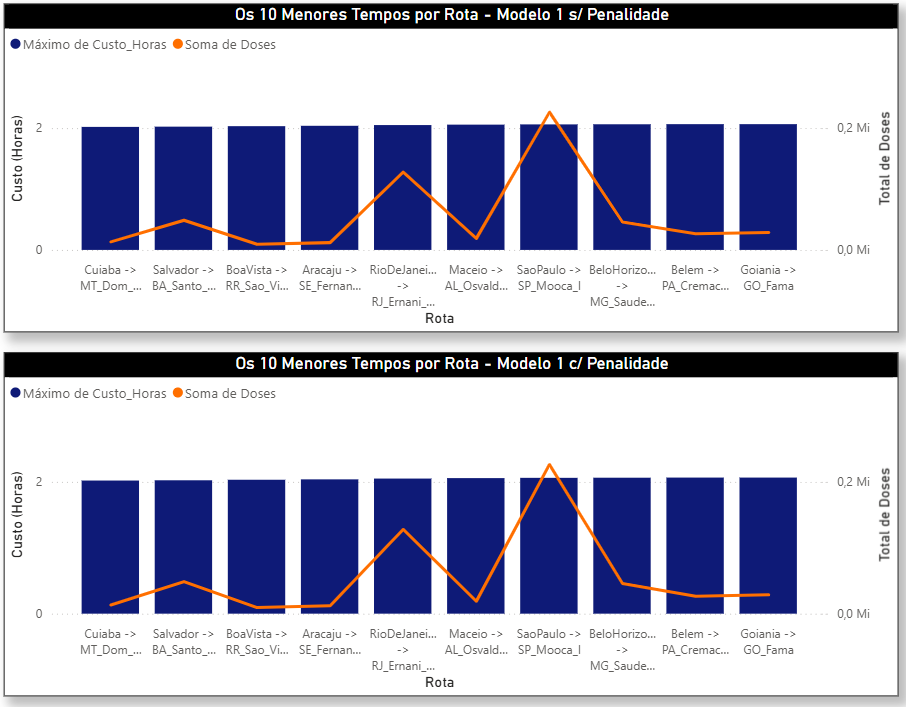
\includegraphics[width=16.0cm,height=12.5cm]{figuras/11-menores_tempos_mod1.png} 
    \legend{Fonte: Elaborado pelo autor (2026)}
    \label{fig:grafico14_powerbi}
\end{figure}

Diferentemente do que ocorre no gráfico de maiores tempos, a análise das rotas mais rápidas revela que a introdução da penalidade de perecibilidade não altera a configuração logística da base da rede. Em ambos os cenários (com e sem penalidade), o conjunto das 10 rotas mais curtas é rigorosamente idêntico.

Observa-se que todas as rotas listadas são exclusivamente intramunicipais (fluxos do tipo $j \to p$), conectando as capitais aos seus respectivos postos de vacinação locais. O eixo de custo em horas apresenta um comportamento estático, formando uma barreira alinhada em, aproximdamente, 2 horas para todas as colunas. Esse fenômeno é explicado pela formulação matemática: como a distância geográfica dentro do mesmo município é muito curta, o custo total da rota passa a ser dominado pelo tempo fixo de processamento logístico do modal rodoviário ($\delta^{rod} = 2,0$ horas).

Os picos de volumes de doses em grandes centros populacionais (como São Paulo e Rio de Janeiro) indicam que estes locais recebem volumes massivos de doses, pois duas demandas são maiores.

\begin{figure}[H]
    \centering
    \caption{Percentual de Tipos de Rota - Modelo 1}
    
\includegraphics[width=16cm,height=5.5cm]{figuras/7-percentual_rotas_mod1.png} 
    \legend{Fonte: Elaborado pelo autor (2026)}
    \label{fig:grafico11_powerbi}
\end{figure}

Verifica-se predomínio, em, aproximadamente 75\%, das rotas do tipo $jp$ ($j \to p$), na qual o município realiza o abastecimento de seus postos. O restante (aproximadamente 25\%) é preenchido pelas rotas do tipo $ij$ ($i \to j$), o que corresponde a casos em que um município precisou pegar doses da oferta de outro município.

Vacina do maior tempo de entrega e rotas gargalo por etapa:

\begin{figure}[H]
    \centering
    \caption{Informações do Terminal Com Python - Modelo 1 sem penalidade}
    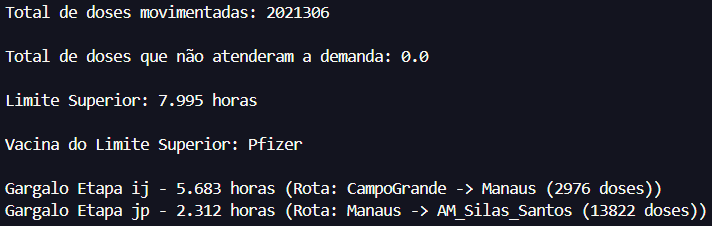
\includegraphics[width=13.5cm,height=5.0cm]{figuras/modelo_1_false.png} 
    \legend{Fonte: Elaborado pelo autor (2026)}
    \label{fig:terminal7_python}
\end{figure}

\begin{figure}[H]
    \centering
    \caption{Informações do Terminal Com Python - Modelo 1 com penalidade}
    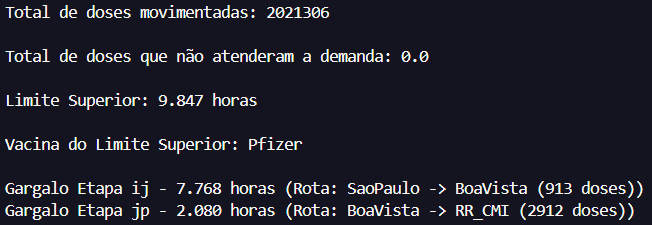
\includegraphics[width=13.5cm,height=5.0cm]{figuras/modelo_1_true.png} 
    \legend{Fonte: Elaborado pelo autor (2026)}
    \label{fig:terminal8_python}
\end{figure}

Verifica-se que rotas gargalo e seus detalhamentos são completamente diferentes entre uma versão de modelo sem penalidade e sua versão com penalidade. O tipo de vacina da entrega mais demorada é a mesma entre as duas saídas. Todas as demandas foram atendidas.

Para complementar a análise espacial dos resultados, foram gerados mapas geográficos interativos utilizando a biblioteca \textit{Folium} em Python. Esses mapas permitem a visualização vetorial das rotas ativas, a distinção dos modais de transporte e a representação do volume de doses transportadas por meio da espessura das arestas. As versões interativas estão hospedadas online e podem ser acessadas nos links: 

\begin{itemize}
    \item Cenário sem penalidade: \url{https://mapa-rotas-m1-false.netlify.app};
    \item Cenário com penalidade: \url{https://mapa-rotas-m1-true.netlify.app}.
\end{itemize}

\begin{figure}[H]
    \centering
    \caption{Mapa Geográfico de Distribuição - Modelo 1 sem penalidade}
    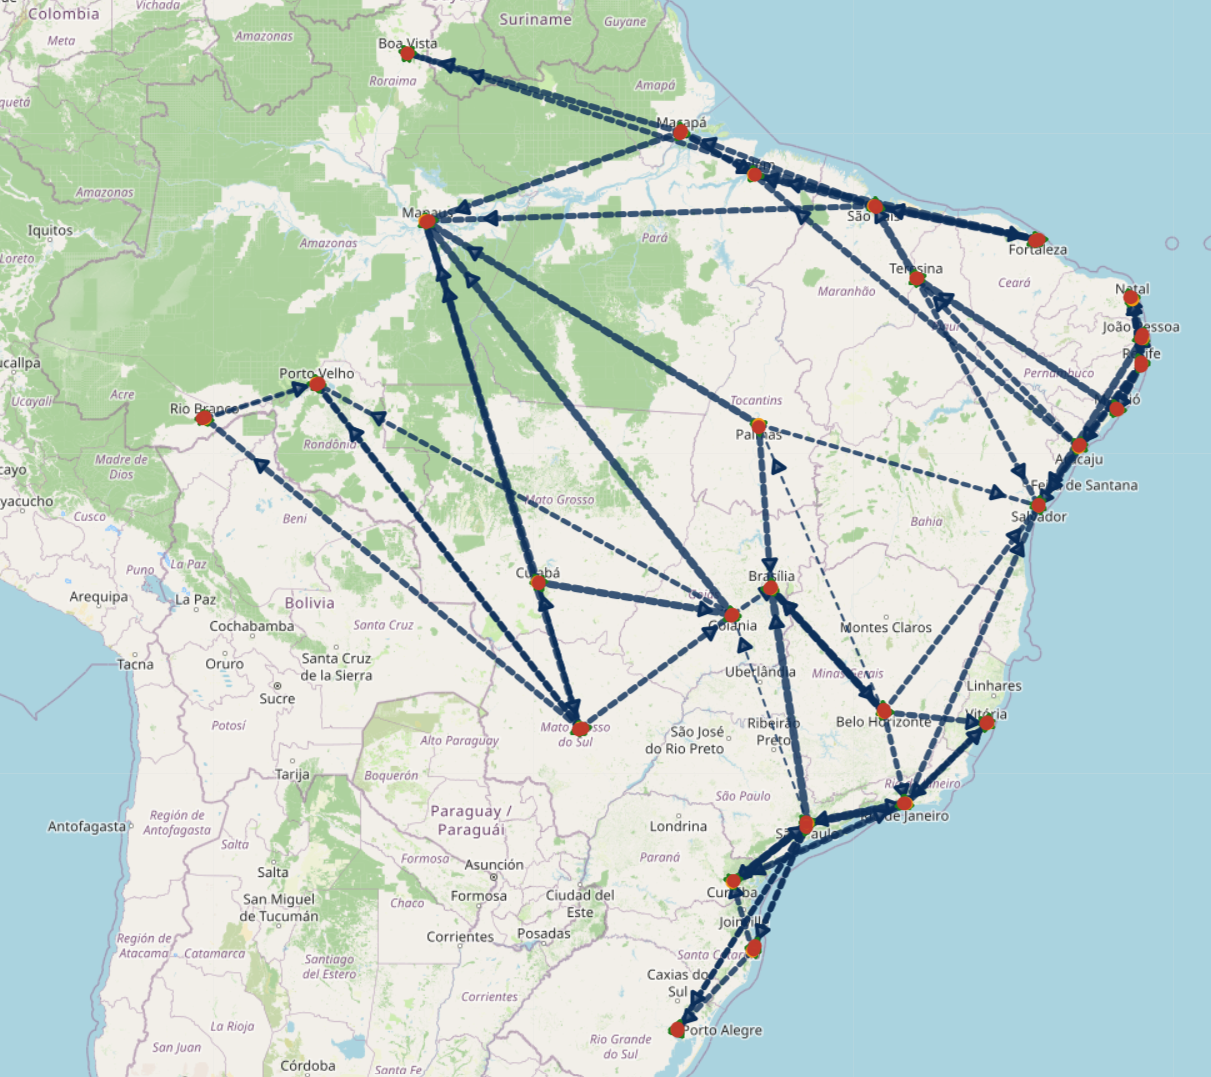
\includegraphics[width=12.0cm,height=12.0cm]{figuras/mapa_m1_false.png} 
    \legend{Fonte: Elaborado pelo autor (2026)}
    \label{fig:mapa_m1_false}
\end{figure}

\begin{figure}[H]
    \centering
    \caption{Mapa Geográfico de Distribuição - Modelo 1 com penalidade}
    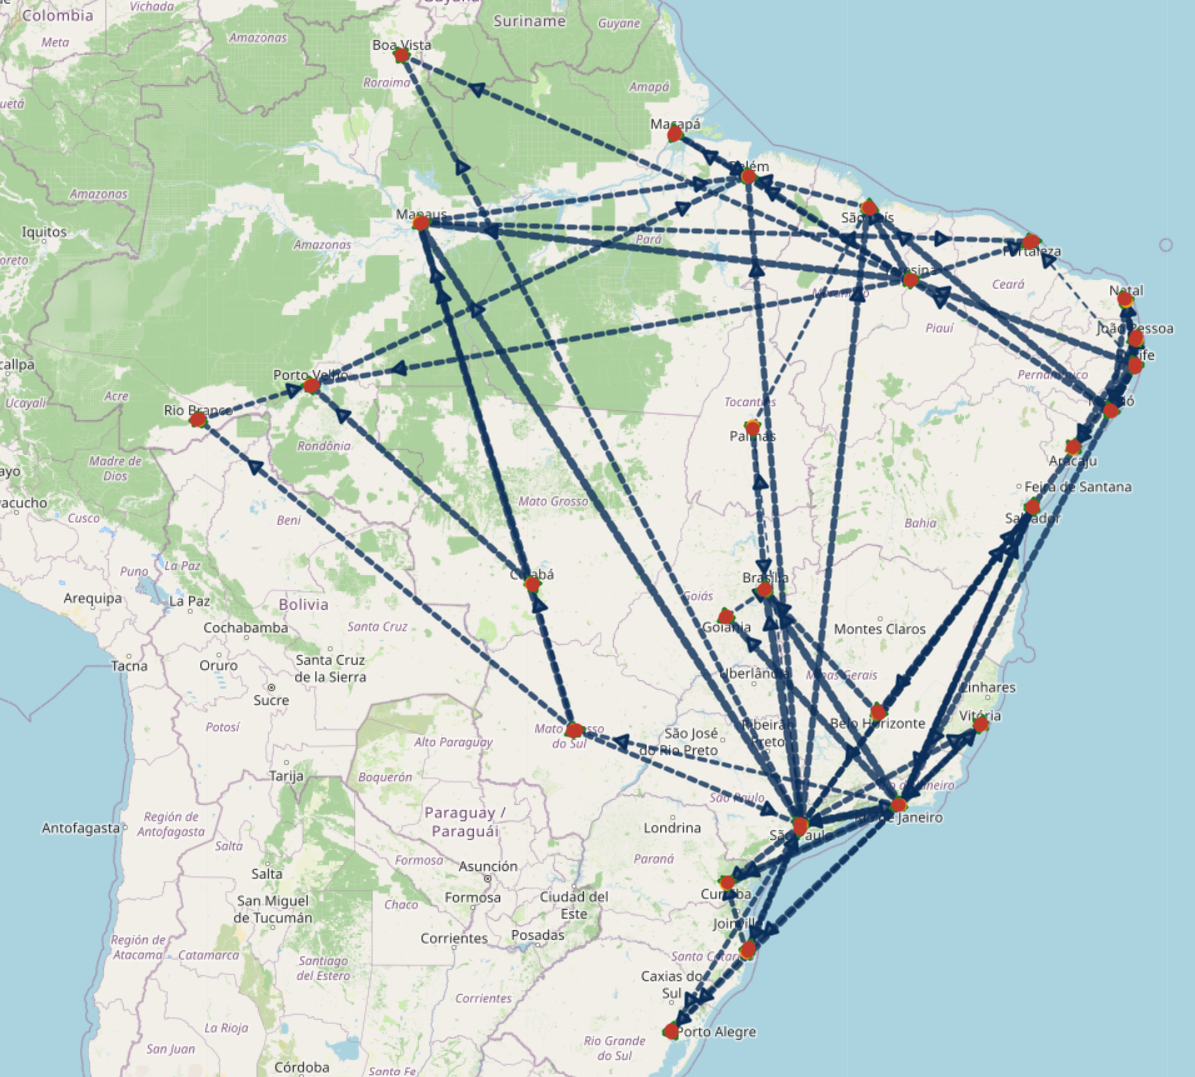
\includegraphics[width=12.0cm,height=12.0cm]{figuras/mapa_m1_true.png} 
    \legend{Fonte: Elaborado pelo autor (2026)}
    \label{fig:mapa_m1_true}
\end{figure}

A análise visual corrobora estritamente os dados quantitativos obtidos. No mapa sem penalidade (Figura \ref{fig:mapa_m1_false}), observa-se uma rede de distribuição mais descentralizada e dispersa pelo território nacional. Em contrapartida, no mapa com penalidade (Figura \ref{fig:mapa_m1_true}), evidencia-se a reestruturação imposta pela pressão de perecibilidade dos lotes: destaca-se visualmente uma forte concentração de vetores aéreos (linhas tracejadas) de longa distância e grande espessura partindo da região Sudeste em direção direta às regiões Norte e Nordeste. Isso consolida a priorização matemática do \textit{solver} em escoar estoques críticos o mais rápido possível por meio do modal aéreo, independentemente da quilometragem física percorrida.

\subsection{Resultados do Modelo 2}

\begin{figure}[H]
    \centering
    \caption{Os 10 Maiores Tempos Por Rota - Modelo 2}
    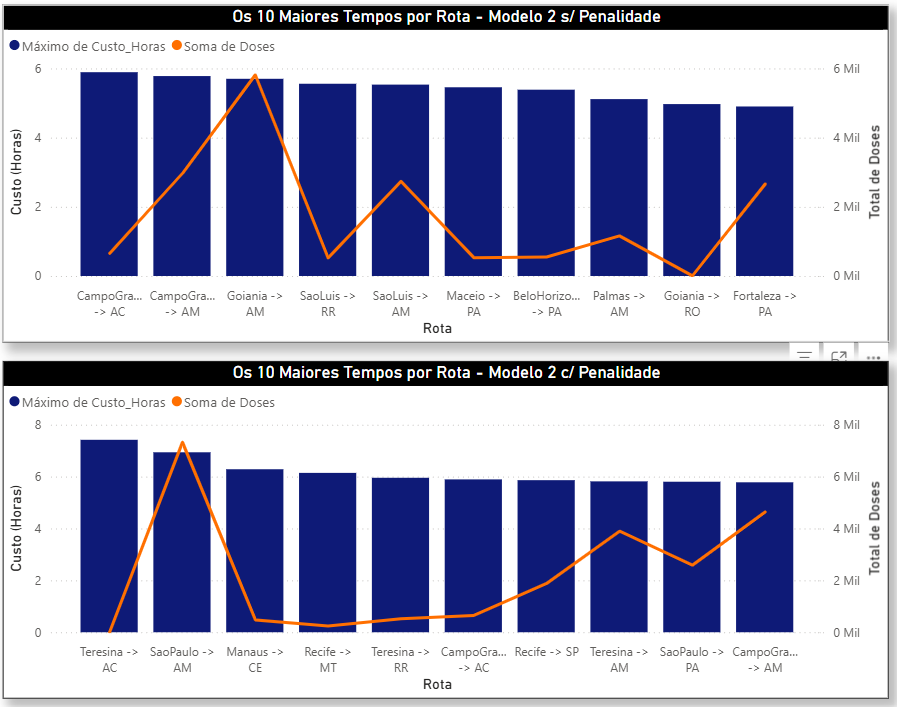
\includegraphics[width=16.0cm,height=12.5cm]{figuras/10-maiores_tempos_mod2.png} 
    \legend{Fonte: Elaborado pelo autor (2026)}
    \label{fig:grafico12_powerbi}
\end{figure}

No cenário sem penalidade, os arcos mais demorados concentram-se no abastecimento de estados da Região Norte e parte do Nordeste a partir do Centro-Oeste e de capitais nordestinas (ex: Campo Grande $\to$ AC, Campo Grande $\to$ AM, Goiânia $\to$ AM, São Luís $\to$ RR). O tempo físico dessas rotas satura de forma homogênea na faixa de 5 a 6 horas.

No cenário com penalidade, o Gurobi reconfigura o topo da lista. Eixos partindo do Nordeste e do Sudeste assumem a liderança crítica (ex: Teresina $\to$ AC, São Paulo $\to$ AM, Manaus $\to$ CE). O solver aceita deliberadamente ativar rotas mais distantes e severas para garantir que os lotes de vacinas com alto risco de vencimento sejam escoados imediatamente de seus polos em direção aos estados receptores. Além disso, na presença da penalidade, o limite do eixo vertical salta de 6 horas para 8 horas.

Da mesma forma que no modelo anterior, o trajeto irregular da linha laranja (Soma de Doses) em ambos os cenários confirma que não há proporcionalidade direta entre o tempo de voo e a quantidade de vacinas transportada.

\begin{figure}[H]
    \centering
    \caption{Os 10 Menores Tempos Por Rota - Modelo 2}
    
\includegraphics[width=16.0cm,height=12.5cm]{figuras/12-menores_tempos_mod2.png} 
    \legend{Fonte: Elaborado pelo autor (2026)}
    \label{fig:grafico15_powerbi}
\end{figure}

A estabilidade frente à penalidade se repete, ou seja, o conjunto das 10 rotas mais curtas é idêntico nos dois casos.

No modelo 2, a diferença estrutural em relação ao Modelo 1 está na composição desse ranking. O gráfico mescla rotas intramunicipais ($j \to p$) com fluxos do tipo $k \to j$ cuja presença decorre de os centros de distribuição estaduais estarem localizados próximos às capitais do mesmo estado.

Nota-se que o tempo fixo de 2 horas do processamento logístico padrão ($\delta^{rod}$) é dominante no custo da rota pelo mesmo motivo apontado na análise feita para o mesmo gráfico do modelo 1.

Novamente, a linha de volume de doses registra picos em entregas à postos locais de capitais populosas e vales em repasses estaduais de menor volume.

\begin{figure}[H]
    \centering
    \caption{Percentual de Tipos de Rota - Modelo 2}
    
\includegraphics[width=16.0cm,height=5.0cm]{figuras/8-percentual_rotas_mod2.png} 
    \legend{Fonte: Elaborado pelo autor (2026)}
    \label{fig:grafico13_powerbi}
\end{figure}

Verifica-se predomínio, em pouco mais da metade, do uso das rotas do tipo $jp$, na qual o município realiza o abastecimento de seus postos. O tipo $ik$ aparece em segundo lugar com aproximadamente 20\% e esse número denota que, na maioria das vezes não foi necessário usar esse tipo de rota tipicamente acionada quando é necessário usar a oferta de outro município. O restante (aproximadamente 15\%) é preenchido pelas rotas do tipo $kj$, na qual o Estado realiza o abastecimento de sua capital. 

Vacina do maior tempo de entrega e rotas gargalo por etapa:

\begin{figure}[H]
    \centering
    \caption{Informações do Terminal Com Python - Modelo 2 sem penalidade}
    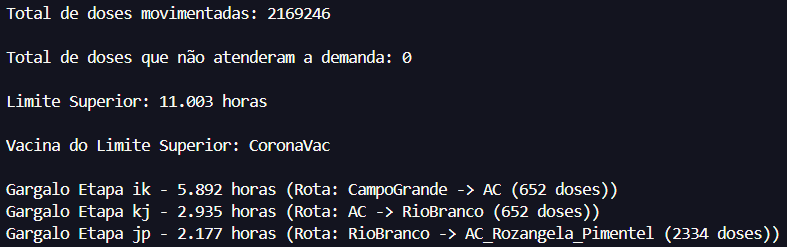
\includegraphics[width=15.0cm,height=5.3cm]{figuras/modelo_2_false.png} 
    \legend{Fonte: Elaborado pelo autor (2026)}
    \label{fig:terminal9_python}
\end{figure}

\begin{figure}[H]
    \centering
    \caption{Informações do Terminal Com Python - Modelo 2 com penalidade}
    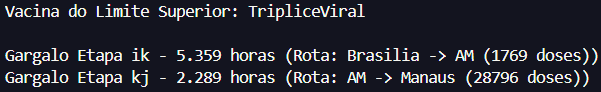
\includegraphics[width=15.0cm,height=5.3cm]{figuras/modelo_2_true.png} 
    \legend{Fonte: Elaborado pelo autor (2026)}
    \label{fig:terminal10_python}
\end{figure}

Exceto pela etapa $ik$, verifica-se que rotas gargalo e seus detalhamentos são exatamente iguais entre uma versão de modelo sem penalidade e sua versão com penalidade. O tipo de vacina da entrega mais demorada é a mesma entre as duas saídas. Todas as demandas foram atendidas.

Também foram gerados mapas geográficos interativos utilizando a biblioteca \textit{Folium} em Python. As versões interativas estão hospedadas online e podem ser acessadas nos links: 

\begin{itemize}
    \item Cenário sem penalidade: \url{https://mapa-rotas-m2-false.netlify.app};
    \item Cenário com penalidade: \url{https://mapa-rotas-m2-true.netlify.app}.
\end{itemize}

\begin{figure}[H]
    \centering
    \caption{Mapa Geográfico de Distribuição - Modelo 2 sem penalidade}
    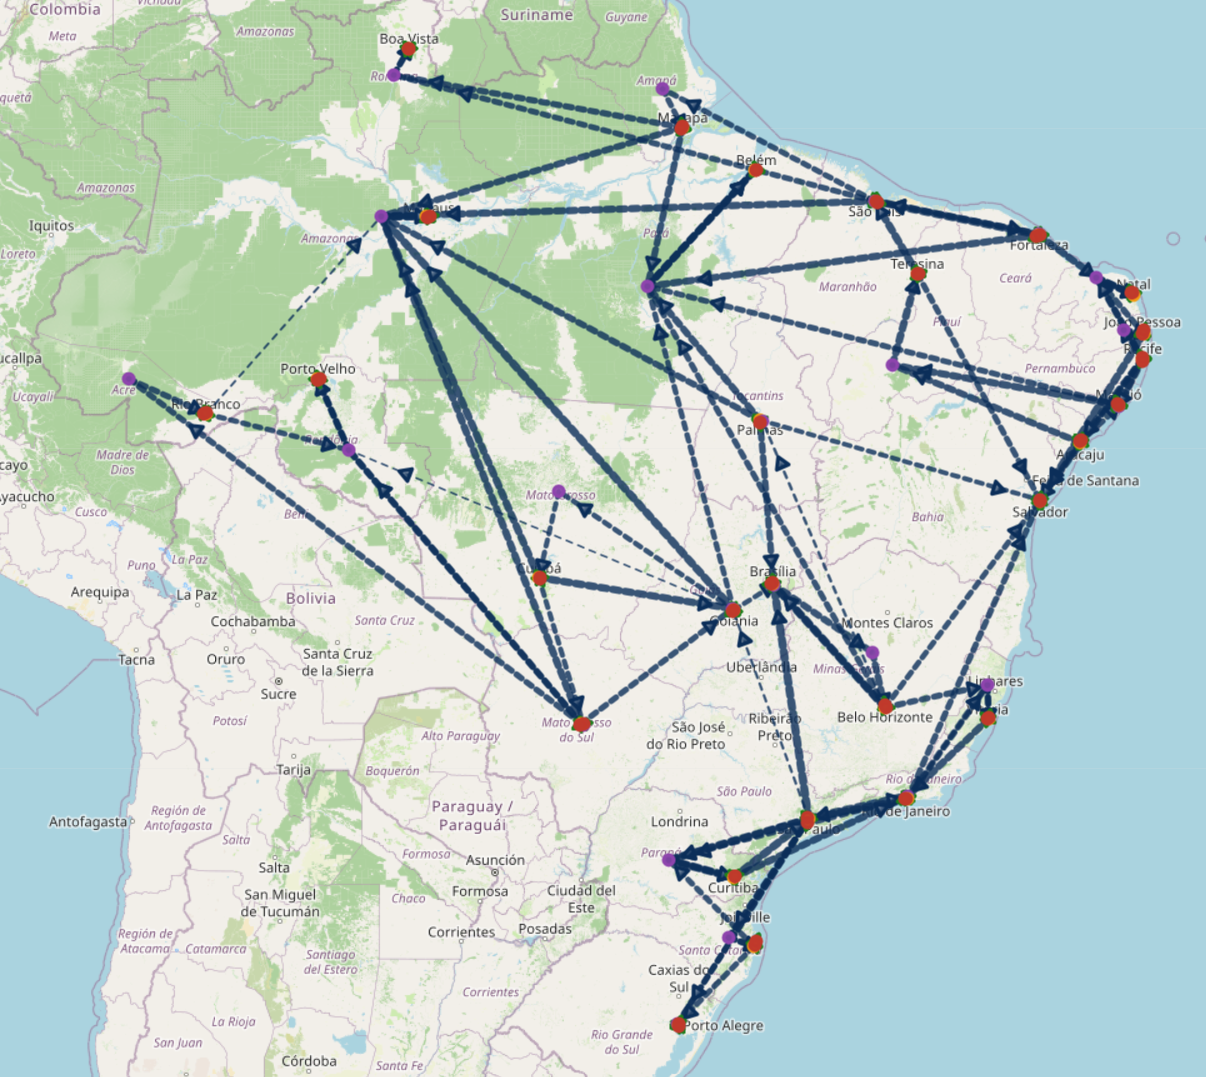
\includegraphics[width=12.0cm,height=12.0cm]{figuras/mapa_m2_false.png} 
    \legend{Fonte: Elaborado pelo autor (2026)}
    \label{fig:mapa_m2_false}
\end{figure}

\begin{figure}[H]
    \centering
    \caption{Mapa Geográfico de Distribuição - Modelo 2 com penalidade}
    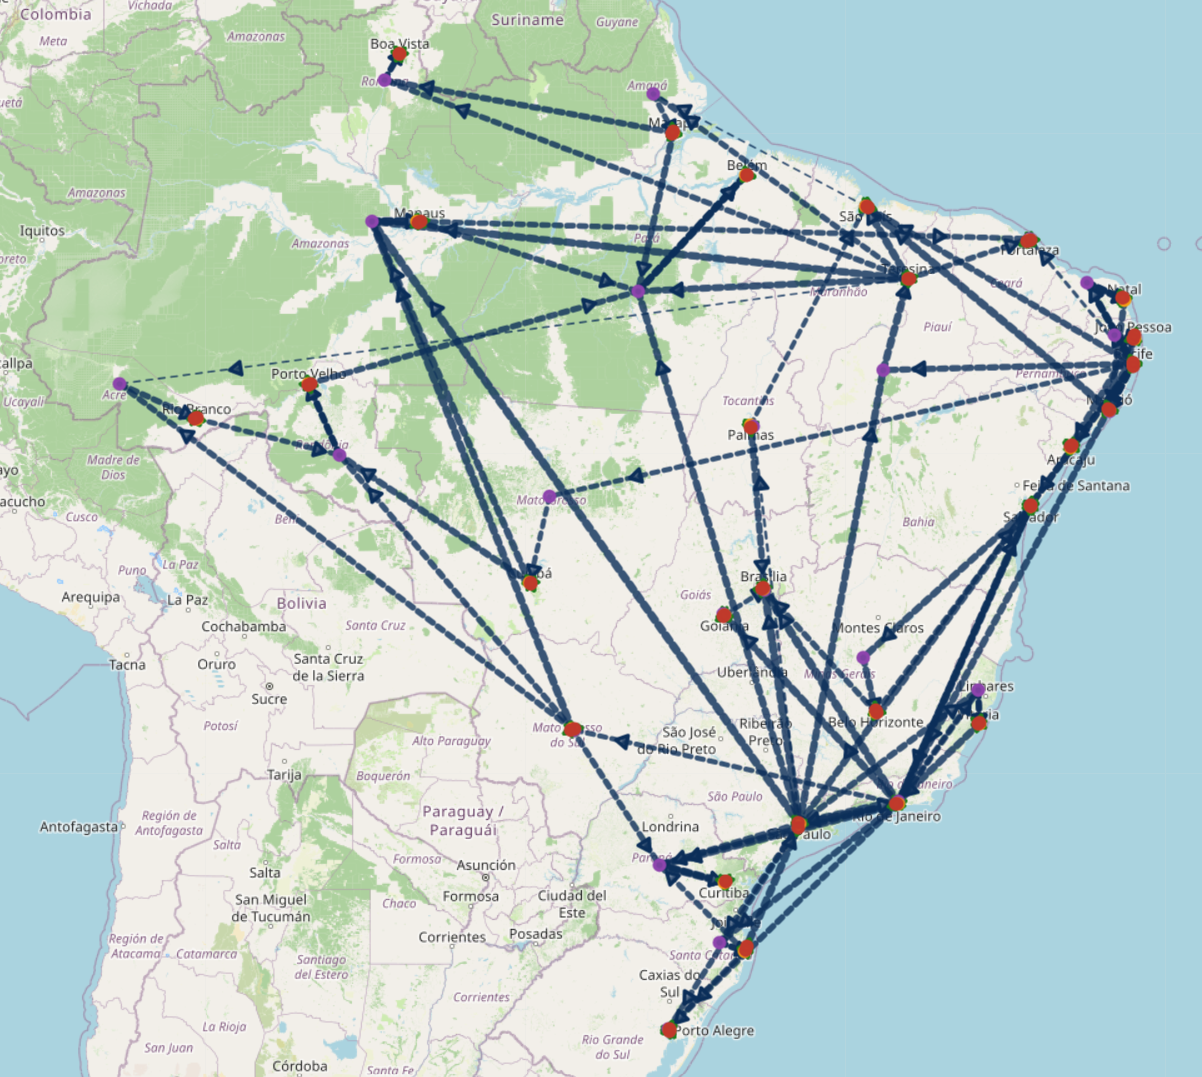
\includegraphics[width=12.0cm,height=12.0cm]{figuras/mapa_m2_true.png} 
    \legend{Fonte: Elaborado pelo autor (2026)}
    \label{fig:mapa_m2_true}
\end{figure}

A análise das rotas dos mapas segue a do modelo anterior: no mapa com penalidade (Figura \ref{fig:mapa_m2_true}), surgem linhas aéreas expressivamente mais longas que no mapa sem penalidade (Figura \ref{fig:mapa_m2_false}), interligando polos distantes do território nacional (como os vetores oriundos do Sudeste e Nordeste rumo à Região Norte). O visual reafirma que a urgência biológica se sobrepõe à lógica da proximidade geográfica, forçando o sistema a ativar rotas de custo elevado para salvaguardar as doses mais críticas da rede antes de sua expiração.

\bigskip